\section{Introduction}
Urban microclimate simulations play a pivotal role in assessing environmental conditions such as pollutant dispersion and thermal behavior within urban areas. These simulations are essential for urban planning, public health, and sustainability efforts.

This document introduces a systematic evaluation methodology aimed at ensuring that computational models can reliably and accurately replicate the physical phenomena relevant to urban environments.

Model evaluation refers to the comprehensive process of determining how well a simulation model represents real-world processes. It encompasses both qualitative and quantitative comparisons between model predictions and empirical observations, and includes aspects such as model validation, performance assessment, and uncertainty quantification.

The validation strategy adopted here employs a hierarchical structure, specifically designed for the Atmospheric Boundary Layer (ABL) with urban micro-scale dynamics. This strategy includes:

\begin{itemize}
    \item Comparisons between simulation outputs and results with relevant observations from wind tunnel and field experiments;
    \item Statistical evaluations of model accuracy;
    \item Sensitivity analyses to assess robustness across model configurations and environmental scenarios.
\end{itemize}

\subsection{Atmospheric Boundary Layer}
ABL is classified into three idealized regimes: Neutrally Stratified Boundary Layer (NSBL), Stable Boundary Layer (SBL), and Convective Boundary Layer (CBL). Each of these regimes is characterized by different stability conditions that significantly influence urban microclimate behavior.

NSBL conditions are most compatible with available wind tunnel datasets but rarely occur in natural settings. SBL and CBL regimes, on the other hand, dominate the diurnal cycle of the urban boundary layer and are better captured in field measurements (and also in some specifically designed wind tunnels).

\begin{figure}[h!]
    \centering
    \begin{minipage}{0.47\textwidth}
        \centering
        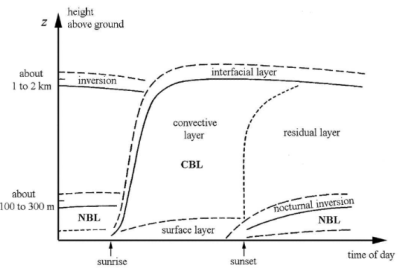
\includegraphics[width=\textwidth]{imgs/abl_cycle.png}
    \end{minipage}
    \hfill
    \begin{minipage}{0.47\textwidth}
        \centering
        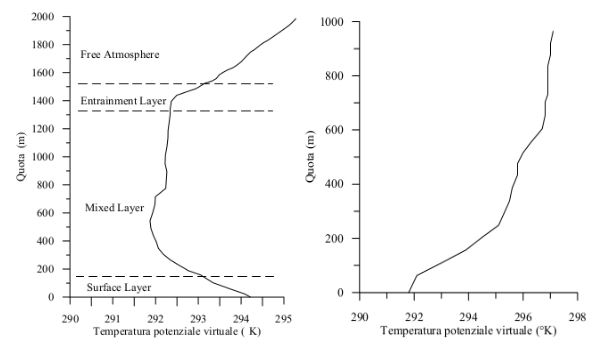
\includegraphics[width=\textwidth]{imgs/wind_speed_cycle.png}
    \end{minipage}
    \caption{Temporal evolution of the ABL and representative wind speed profile across a diurnal cycle.}
\end{figure}

\subsection{CFD Evaluation for Urban Microclimate Simulations}
Computational Fluid Dynamics (CFD) is a key tool for simulating airflow and pollutant dispersion in urban settings. These simulations provide detailed insight into microscale atmospheric behavior, but the reliability of CFD predictions strongly depends on rigorous model validation.

To ensure robustness and credibility, CFD models must be evaluated through a structured process that considers accuracy, computational efficiency, and physical fidelity. The hierarchical validation strategy introduced here supports these objectives by organizing test cases according to geometric complexity and atmospheric conditions.

The methodology leverages test cases derived from well-documented datasets, enabling focused evaluation of specific flow features and physical processes. Key goals of this strategy include:

\begin{itemize}
    \item Establishing a balance between computational cost and predictive accuracy;
    \item Validating models under different configurations of the ABL;
    \item Testing performance on canonical unit problems, such as flow over isolated buildings, through street canyons, and within complex topographies.
    \item Testing performance on real-world scenarios, such as urban areas with complex geometries and varying atmospheric conditions.
\end{itemize}

\noindent
Above-mentioned unit problems are designed to represent simplified, yet physically meaningful, urban scenarios in which buildings and other geometrical features are fully immersed in a turbulent boundary layer with dispersion of gaseous substances. The following categories are used:

\begin{itemize}
    \item Flow field around a \textbf{single building};
    \item Flow field within a \textbf{street canyon};
    \item \textbf{Dispersion} of neutrally and non-neutrally buoyant substances;
    \item Flow around \textbf{complex urban topographies}.
\end{itemize}

\begin{figure}[h!]
    \centering
    \begin{minipage}{0.44\textwidth}
        \centering
        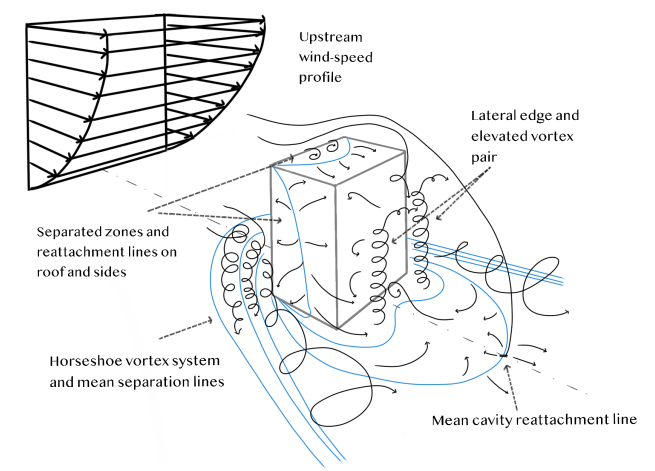
\includegraphics[width=\textwidth]{imgs/unit_problem_2.png}
    \end{minipage}
    \hfill
    \begin{minipage}{0.44\textwidth}
        \centering
        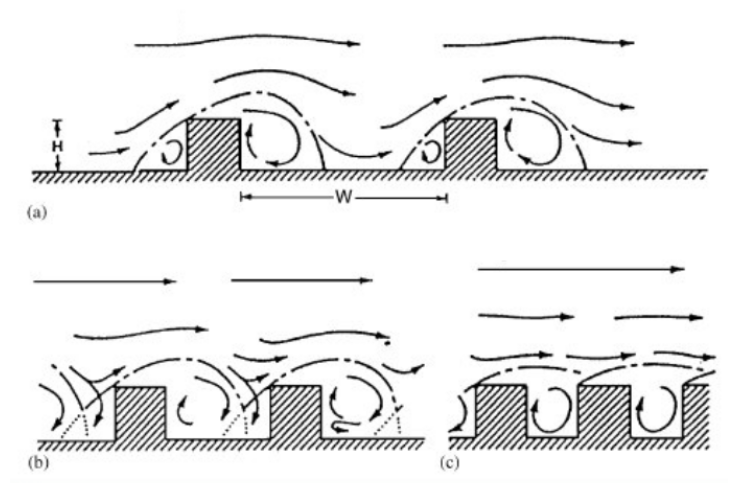
\includegraphics[width=\textwidth]{imgs/unit_problem_1.png}
    \end{minipage}
    \caption{Illustration of unit problems representing key physical phenomena in urban microclimates.}
\end{figure}
